\documentclass[12pt]{article}
\usepackage{graphicx}
\renewcommand{\baselinestretch}{1.5}
%\usepackage{indentfirst}

\begin{document}

\section{Xie algorithm}

This watermarking technique \cite{xie1} operates within the discrete wavelet transform (DWT) domain. It 
is an oblivious watermarking scheme that inserts a signature $w_{i}$, where $w_{i} \in \{0,1\}$.
The method operates only upon the low frequency subband of the DWT, quantizing 
the median of a local area to a value determined by its neighbours.

\subsection{Watermark insertion}
A $1 \times 3$ non-overlapping window is run across the low frequency approximation subband. 
One of these three coefficients is selected and manipulated in a non-linear fashion 
in order to insert a watermark bit. Figure \ref{slidingWin} illustrates this process.

\begin{figure}[htb]
	\begin{center}
		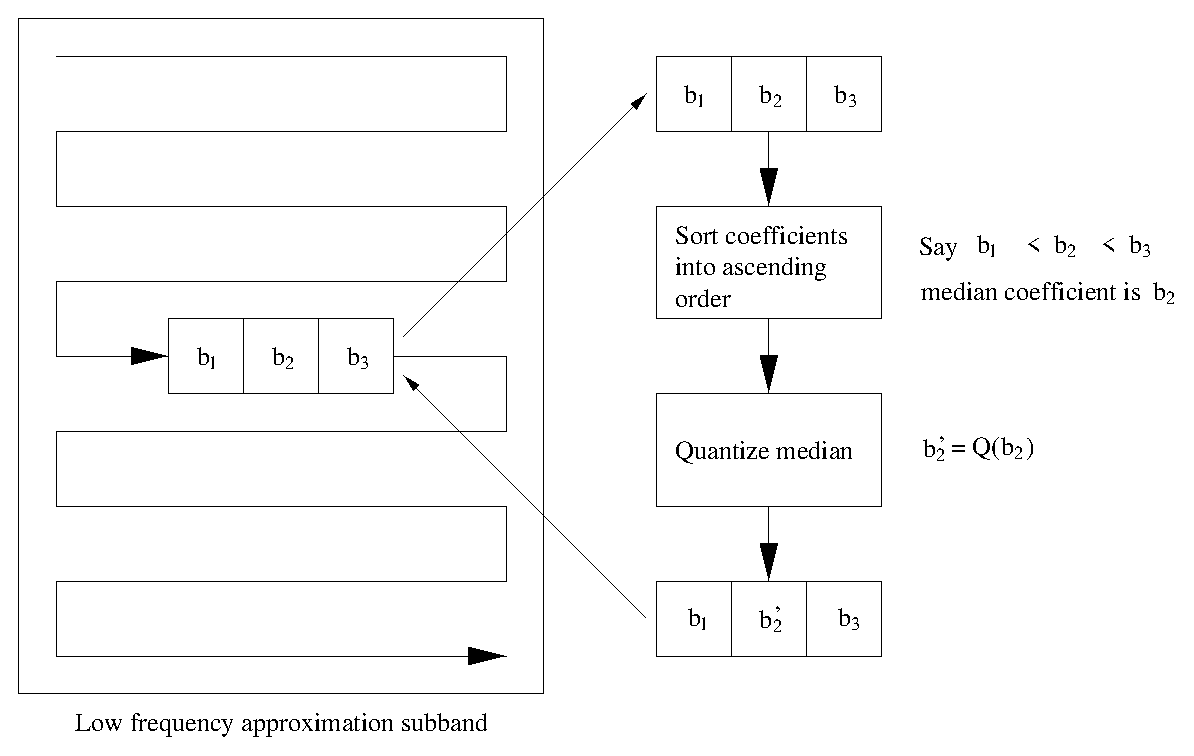
\includegraphics[height=8cm,width=12.8cm]{slidingWinNoAbs.pstex}
		\caption{Running a non-overlapping $1 \times 3$ window over the low frequency
			subband in order to select a coefficient which to quantize to 
			embed a watermark.}
		\label{slidingWin}
	\end{center}
\end{figure}

Firstly, the three elements from the non-overlapping sliding window ($b_{1}, b_{2}$ and $b_{3}$) are sorted into 
ascending order according
to their magnitudes. The range between the maximum value and the minimum value is split into
intervals according to:
\begin{equation}
	S_{\alpha} = \alpha \frac{ \mbox{max}|b_{i}| - \mbox{min}|b_{i}| }{2}
\end{equation}
where $b_{i} \in \{b_{1}, b_{2}, b_{3}\}$. Thus, the total number of intervals, $M$, is given by:
\begin{equation}
	M = \frac{2}{\alpha}
\end{equation}

Each of these $M$ intervals has two boundaries, $l_{k}$ and $l_{k+1}$. One of these boundaries will be odd
while the other will be even. Figure~\ref{fig-quantizing} shows how a watermark bit is embedded via quantization.
\begin{figure}[hbt]
        \begin{center} 
                \includegraphics[height=2cm,width=12.2cm]{quantizing.pstex} 
		\caption{Quantizing the median pixel ($b_{2}$) to a value represented by an odd or an even boundary.
			In this example, $l_{k}$ is assumed to be an odd boundary.}
		\label{fig-quantizing}
	\end{center}
\end{figure}  
In this figure, two examples of $b_{2}$ are given (note that $b_{2}$ is the magnitude of the median pixel from 
the $1 \times 3$ sliding window). The pixel with the mimimum magnitude is $b_{1}$ and the pixel with the 
maximum magnitude is $b_{3}$. Between $b_{1}$ and $b_{3}$, there are $M$ intervals, $l_{0}, l_{1} ... l_{M}$.
A watermark bit value of one is associated to all the even boundaries and a watermark bit value of zero 
is associated to all the odd boundaries. The $l_{k}$ boundary in figure \ref{fig-quantizing} is assumed to be odd
(\emph{i.e.}, $k$ is odd).
Thus, to embed a watermark bit of one, the $b_{2}$ value that lies within $[l_{k-1},l_{k}]$ would
be quantized to have the same magnitude as $l_{k-1}$ and the $b_{2}$ value that lies within $[l_{k},l_{k+1}]$
would be quantized to have the same magnitude as $l_{k+1}$. Both of the $b_{2}$ values would be quantized to 
have the same magnitude as $l_{k}$ if a watermark bit of zero were to be embedded.
These boundaries are also termed reconstruction points as they are part of the output set of the quantizer 
which are used in the watermark extraction process.

\subsection{Watermark detection}
The possibly watermarked image is decomposed to obtain the low frequency approximation subband of the DWT.
An non-overlapping $1 \times 3$ window is run across this entire subband, as detailed in figure \ref{slidingWin}.
The median of all these windows is calculated and then quantized to lie on a reconstruction point. 
The bit value associated with this reconstruction point (boundary) is the recovered watermark value.





			
\begin{thebibliography}{00}
	\bibitem{xie1}L. Xie and G. R. Arce, Joint wavelet compression and authentication
	watermarking, \emph{Proceedings of the IEEE International Conference on Image Processing, ICIP'98}, 
	Volumne 2, Chicago, IL, USA, 1998, 427-431.
\end{thebibliography}

\end{document}
